% This must be in the first 5 lines to tell arXiv to use pdfLaTeX, which is strongly recommended.
\pdfoutput=1
\documentclass[11pt]{article}
\usepackage{EMNLP2023}

\usepackage{times}
\usepackage{latexsym}
\usepackage[T1]{fontenc}
\usepackage[utf8]{inputenc}
\usepackage{microtype}
\usepackage{inconsolata}
\usepackage{url}
\usepackage{booktabs}
\usepackage{graphicx}
\usepackage{float}
\usepackage{enumitem}

\title{Kaggle Competition Report: Language Identification via Text Classification}

\author{
    Abdellah Oumida, Elisa Faure, Idriss Mortadi, Marianne Brugidou \\
    CentraleSupélec, France \\
    \texttt{\{abdellah.oumida, elisa.faure, idriss.mortadi, marianne.brugidou\}@student-cs.fr}
}



\begin{document}
\maketitle

\begin{abstract}
This report outlines our approach for the Advanced NLP Class Kaggle Competition, which involves predicting the language of a given text using the ISO-639-3 standard. Our solution employs the \texttt{xlm-roberta-base} model with parameter-efficient fine-tuning (LoRA), complemented by data augmentation and a cosine annealing scheduler. This method achieved a leaderboard score of \textbf{0.87996}.

\section{Introduction}
Language identification is a crucial preprocessing step in many NLP applications. The Advanced NLP Class Kaggle Competition requires classifying a given text into one of 389 languages or dialects, which form a curated subset of the ISO-639-3 standard \citep{iso639-3}. This high-granularity classification presents challenges due to the large label space and diverse linguistic features. Our approach leverages a pre-trained multilingual transformer model, adapted through Low-Rank Adaptation (LoRA) \citep{hu2022lora}, to address these challenges efficiently.

\section{Solution}
Our solution consists of several key components:
\subsection{Preprocessing}
Our text preprocessing pipeline is designed to clean and normalize text data efficiently.
We developed a custom dataset \textbf{class} to read CSV files, tokenize texts with the HuggingFace tokenizer, and apply data augmentation. Specifically, any text exceeding 128 tokens is truncated or randomly sliced (if \texttt{AUGMENT} is enabled) to improve generalization, especially for low-resource languages. Then we proceed to clean the dataset.

The first step involves script detection and filtering, where we use Unicode codepoint ranges to identify the script of each character in the text. By leveraging a lookup table from "unicode\_ranges.csv", we map Unicode ranges to specific language groups. To optimize performance, we employ a binary search ("bisect") to determine the script of each character and maintain a frequency count of detected scripts. Once the majority script is identified, the function "filter\_majority\_script" ensures text uniformity by retaining only characters that belong to the most frequently occurring script in the input text.  

In addition to script filtering, we remove unnecessary elements such as URLs, tags, and hashtags. The function `remove\_links\_and\_tags` eliminates links that start with `http://`, `https://`, or `www.`, as well as tags that begin with `@` and hashtags that start with `\#`. To enhance readability, multiple consecutive spaces are reduced to a single space.  

By implementing these preprocessing steps, our approach ensures that the text is clean, consistent, and free from unnecessary, making it more suitable for training our models.


\subsection{Training}
In Kaggle's cloud environment, we have access to two NVIDIA Tesla T4 GPUs \citep{nvidiaT4}. Each T4 GPU features 2,560 CUDA cores and 16 GB of GDDR6 memory. By leveraging Hugging Face's Accelerate library \citep{accelerate}, we can efficiently train large-batch models using these GPUs.

\begin{itemize}[leftmargin=*]
    \item \textbf{Model Architecture:} We build upon a fine tuned version of \textbf{xlm-roberta-base} we found on HuggingFace: \textbf{papluca/xlm-roberta-base-language-detection}\footnote{\href{https://huggingface.co/papluca/xlm-roberta-base-language-detection}{papluca/xlm-roberta-base-language-detection}}, an XLM-RoBERTa variant fine-tuned for language identification. It relies on the XLM-RoBERTa architecture \citep{conneau2020unsupervised} with a classification head on top (i.e., a linear layer over the pooled output). This model can be used directly as a language detector for 20 languages, including Arabic, English, French, Hindi, and Chinese, among others. We integrate LoRA \citep{hu2022lora} via the PEFT framework \citep{peft}, updating only the query and value modules in the transformer blocks. This parameter-efficient approach substantially reduces the number of trainable parameters, which is particularly beneficial given the large number of language classes.
    
   
    
    \item \textbf{Data Processing:} We set the maximum sequence length to 128 tokens. Random slicing is applied for texts exceeding 128 tokens to diversify the training examples.
    
    \item \textbf{Training:} We train for 40 epochs with a learning rate of 6e-3 and weight decay of 0.01. Large batch sizes (320 samples per device) ensure stable gradient estimates. We use the AdamW optimizer with a learning rate scheduler that employs cosine annealing with warm restarts, where \( T_0 = 20 \), \( T_{\text{mult}} = 2 \), and \( \eta_{\text{min}} = 1\text{e-4} \).  We log training metrics every 100 steps.
    
    \item \textbf{LoRA parameters:}
    We use LoRA (Low-Rank Adaptation) for efficient fine-tuning. Key parameters include:

    \begin{itemize}
        \item \textbf{Rank (\texttt{r})}: 8, rank of LoRA update matrices.
        \item \textbf{Scaling Factor (\texttt{lora\_alpha})}: 32, scales LoRA updates.
        \item \textbf{Dropout (\texttt{lora\_dropout})}: 0.1, prevents overfitting.
        \item \textbf{Target Modules}: \texttt{"query"} and \texttt{"value"}.
    \end{itemize}

    
\end{itemize}

\section{Results and Analysis}
\begin{table}[H]
\centering
\setlength{\tabcolsep}{2pt}
\begin{tabular}{lccc}
\toprule
\textbf{Metric} & \textbf{Precision} & \textbf{Recall} & \textbf{F1-score} \\
\midrule
Macro Average & 0.88 & 0.88 & 0.88 \\
Weighted Average & 0.88 & 0.87 & 0.87 \\
\bottomrule
\end{tabular}
\caption{Overall evaluation metrics on the validation set.}
\label{tab:metrics}
\end{table}

We evaluated our model on a held-out validation set, achieving an overall accuracy of 0.88. Table~\ref{tab:metrics} shows the macro and weighted average metrics, both indicating strong performance across classes. However, a detailed classification report revealed that while certain languages (e.g., \texttt{abk}, \texttt{ace}, \texttt{ach}) reached near-perfect scores, others (e.g., \texttt{acm}, \texttt{afb}) performed less consistently, suggesting a need for further optimization for low-resource or highly similar dialects.

\begin{figure}[H]
    \centering
    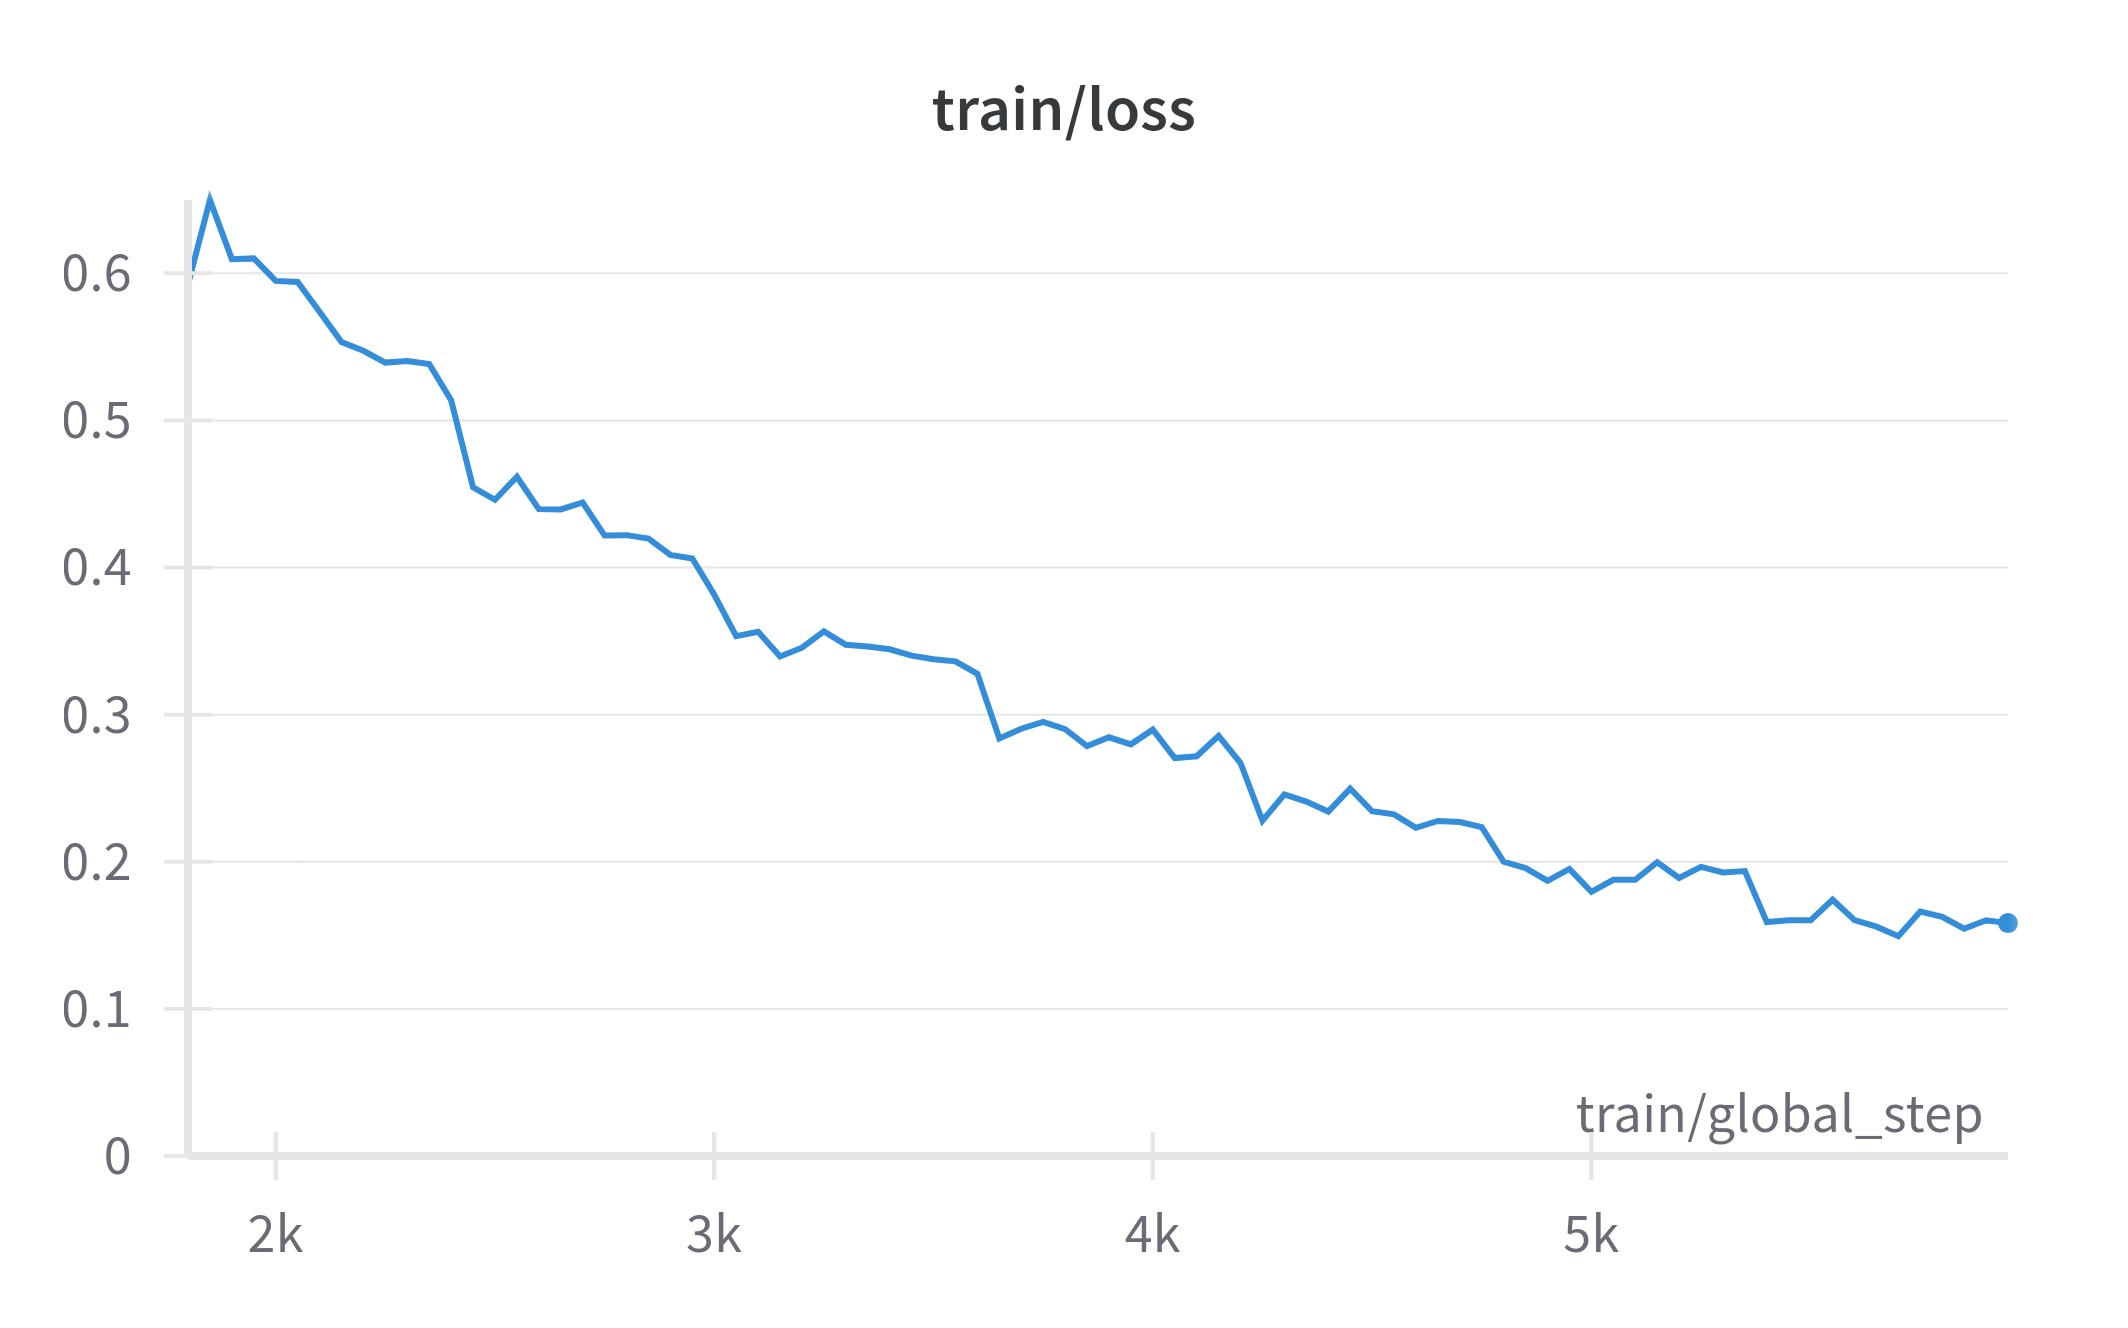
\includegraphics[width=0.45\textwidth]{figures/new_ANLP_kaggle_validation_loss_over_epochs.png.png}
    \caption{Validation loss over training steps.}
    \label{fig:val_loss}
\end{figure}

\begin{figure}[H]
    \centering
    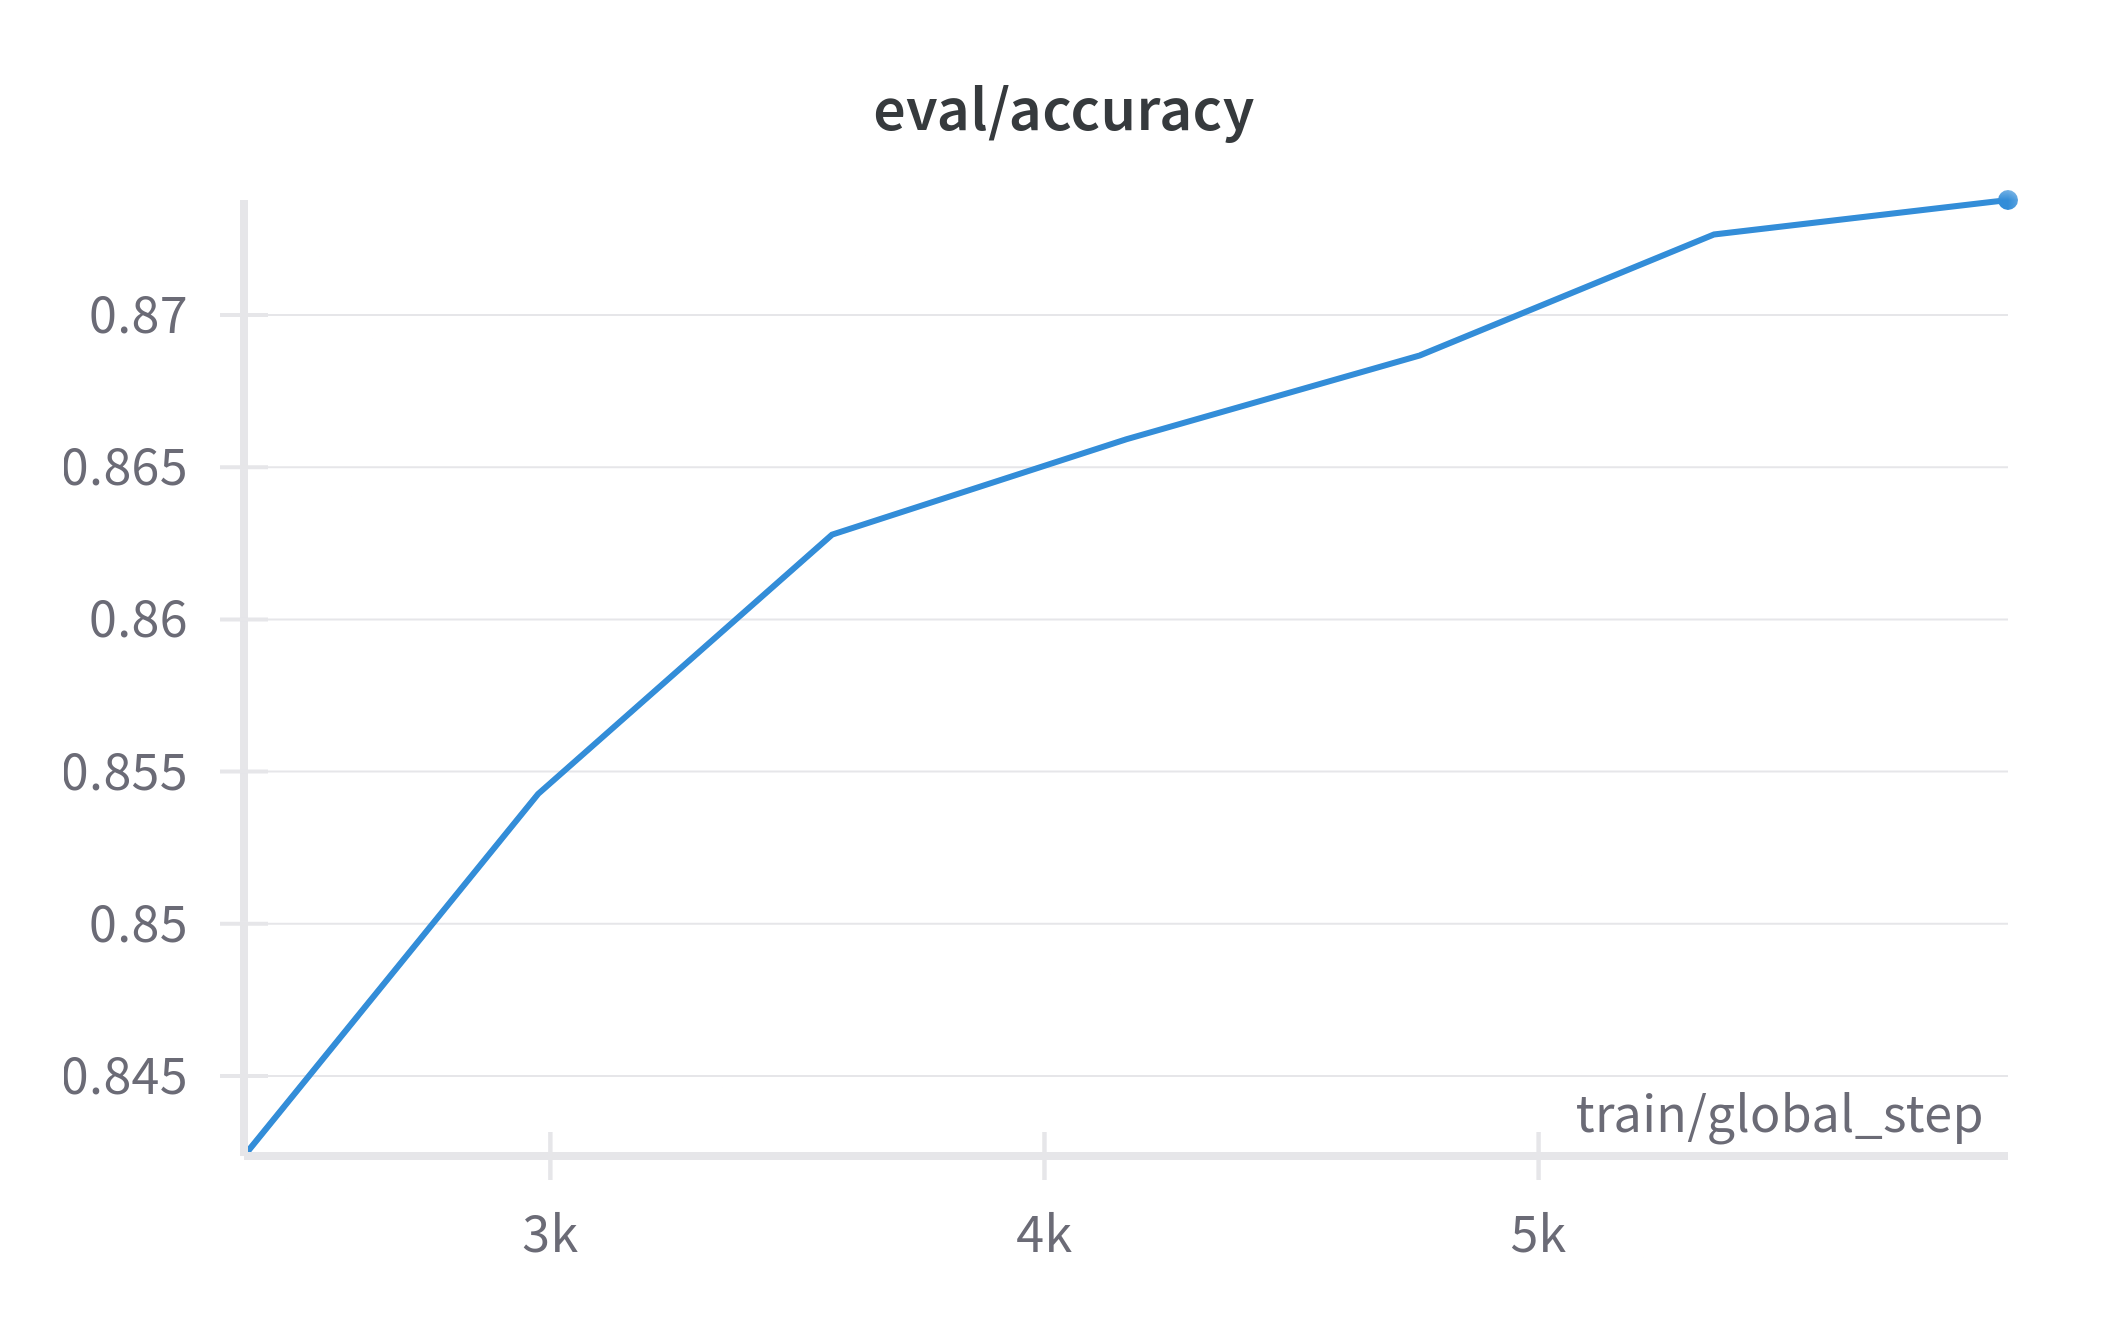
\includegraphics[width=0.45\textwidth]{figures/new_ANLP_kaggle_validation_accuracy_over_epochs.png}
    \caption{Validation accuracy over training steps.}
    \label{fig:val_accuracy}
\end{figure}

Figures~\ref{fig:val_loss} and \ref{fig:val_accuracy} illustrate the validation loss and accuracy trends across epochs. The validation loss decreases steadily down to 0.15, while the accuracy improves from up to 0.87, indicating consistent learning progress. These curves suggest that the chosen hyperparameters and learning rate schedule allowed for stable training without noticeable overfitting.

\section*{Limitations}

We initially attempted full fine-tuning but were limited by time and computational resources. Instead, we used LoRA for efficiency, though it has trade-offs. Our model's fixed maximum sequence length may affect performance on longer inputs. Evaluation was done on a single pre-trained model and data split. Ensemble methods and further hyperparameter tuning could improve performance, especially for underrepresented languages.

\bibliographystyle{acl_natbib}
\bibliography{custom}

\end{document}